\documentclass[11pt,final]{article}
\renewcommand*\familydefault{\sfdefault}
%\usepackage{amssymb,amsmath,amsfonts,comment}
%\usepackage{amsmath,amssymb,graphicx,subfigure,psfrag}
\usepackage{amsmath,amssymb,graphicx,subfigure,psfrag,upgreek}
\usepackage{algorithm,algorithmic}
\usepackage{amssymb,mathrsfs}
\usepackage[margin=1in]{geometry}
\usepackage{parskip}
\usepackage{graphicx}
\usepackage{bm}
\usepackage{color,pdfcolmk}
\usepackage{enumitem,kantlipsum}
\newcommand{\todo}[1]{\noindent\emph{\textcolor{red}{Todo: #1\:}}}
%\newcommand{\alennote}[1]{\noindent\emph{\vspace{1ex}\textcolor{cyan}{Alen: #1\:}}\\[1ex]}
\newcommand{\referee}[1]{\vspace{.1ex}\noindent{\textcolor{blue}{#1}}}



\begin{document}

%We thank the reviewers for their careful reading of our article 
%and the helpful comments and suggestions.
%Please find below point-by-point replies (in black) to your comments and
%questions (which are reprinted in blue). To give you an overview of all the
%changes in the paper, we also provide a diff-document that highlights the
%changes between the initial submission and this re-submission.\\[1ex]
\begin{center}
{\bf Summary of Modifications to CNF-D-18-00757}\\[6pt]
{\bf Subspace-based dimension reduction for chemical kinetics applications with 
epistemic uncertainty}\\[6pt]
By \\
Manav Vohra, Alen Alexanderian, Hayley Guy, Sankaran Mahadevan 
\end{center}

%\baselineskip=22pt


\vspace*{1in}

We are once again thankful to the reviewers for their positive feedback on the revised 
manuscript. Through this response, we sincerely hope to have addressed the
outstanding issues and concerns. 
A point-by-point
response to the comments has been provided as follows. Corresponding modifications
where appropriate, have been highlighted (in blue) in the revised manuscript. 

\clearpage


\section*{Reviewer \#1}

\begin{enumerate}[wide, labelwidth=!, labelindent=0pt]
\item \referee{I recommend accepting the manuscript, provided that the authors explore and provide evidence (to this 
Reviewer at least) that the applicability and conclusions on the method's performance do not change when the initial 
temperature and pressure are such that the ignition delay time falls in the 0.1 to 1 ms range, which is 2 to 3 orders of 
magnitude lower than the ignition delay time that they have presented.
It is my wish to see the data, perhaps just as a response to me facilitated by the editor, before recommending publication.
Perhaps there has been a misunderstanding. When I pointed to the O(0.1 s) delay time, I did not imply that there was an 
error in the calculation and/or a bug in TChem. What I meant is simply that the initial conditions were likely to be unrealistic.
In the revised revision, the authors mention that the conditions are 1 atm, 900 K, and equivalence ratio of 2.0. These 
conditions, giving an ignition delay time of O(0.1 s) are obviously highly unrealistic and impractical as there is no application 
that may rely on such long ignition delay times.
Conditions (higher pressures/higher temperatures) such that an ignition delay time O(0.1 - 1 ms) are practical and should be 
explored by the authors.
It may very well be that nothing changes in the analysis and conclusions, but then, again, why consider an unrealistic set of 
conditions in the first place$?$
}

We thank the reviewer for this comment and suggestions. In accordance with the reviewer's suggestion, the initial 
temperature~($T_0$) and pressure~($P_0$) was increased to ensure that the ignition delay is in the desired
range, i.e. 0.1--1~ms. Specifically, the nominal values of $T_0$ and $P_0$ were increased from 900~K to 1000~K, and
from 1~atm to 1.5~atm respectively. In keeping with the paper, a 2$\%$ perturbation about these nominal values was used
for the purpose of computing the active subspace. Prior distributions of the equivalence ratio and the rate-controlling
parameters were used as before. In Figure~\ref{fig:kde}, we illustrate the probability density function of the ignition delay
obtained using 10,000 pseudorandom samples in the input domain. 
%
\begin{figure}[htbp]
 \begin{center}
  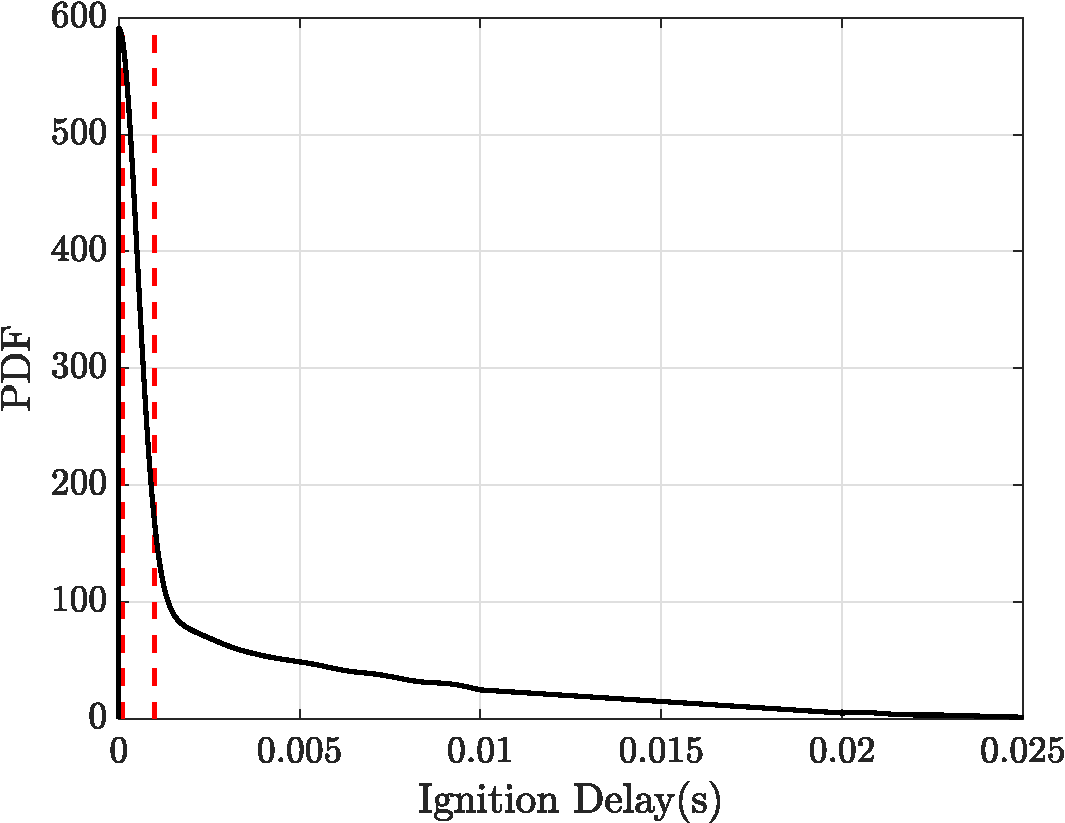
\includegraphics[width=0.40\textwidth]{./Figures/pdf_ign_small}
  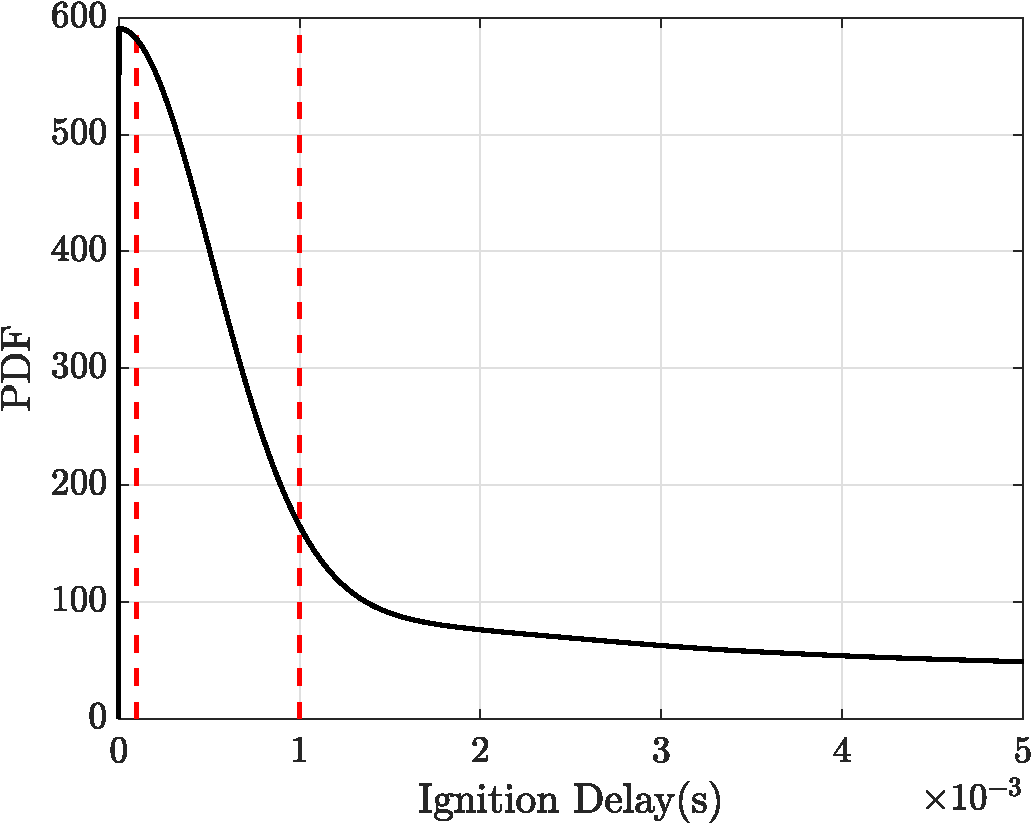
\includegraphics[width=0.38\textwidth]{./Figures/pdf_ign_small_zoom}
\caption{Left: PDF plots generated using kernel density estimation of the ignition delay computed at 10,000 samples.
Right: The same PDF is illustrated using a smaller range in the x-axis to highlight the region of interest, i.e. 0.1~ms--1~ms.
The range of interest is highlighted by the two vertical lines.} 
\label{fig:kde}
\end{center}
\end{figure}
%
As observed in the pdf plots in Figure~\ref{fig:kde}, the bulk of the high probability region is captured by the range of interest
for the ignition delay~(0.1~ms--1~ms), highlighted using the two vertical lines corresponding to the bounds of the interval.
Hence, we consider $P_0=1.5$~atm and $T_0=1000$~K as reasonable
choices for the purpose of this analysis. 

The proposed methodology in the paper was implemented to this new set-up. The regression approach was used for
estimating the gradient using model evaluations at 500 samples. In Figure~\ref{fig:as}, we illustrate the
eigenvalue spectrum~(left), and the sufficient summary plot~(right).
%
\begin{figure}[htbp]
 \begin{center}
  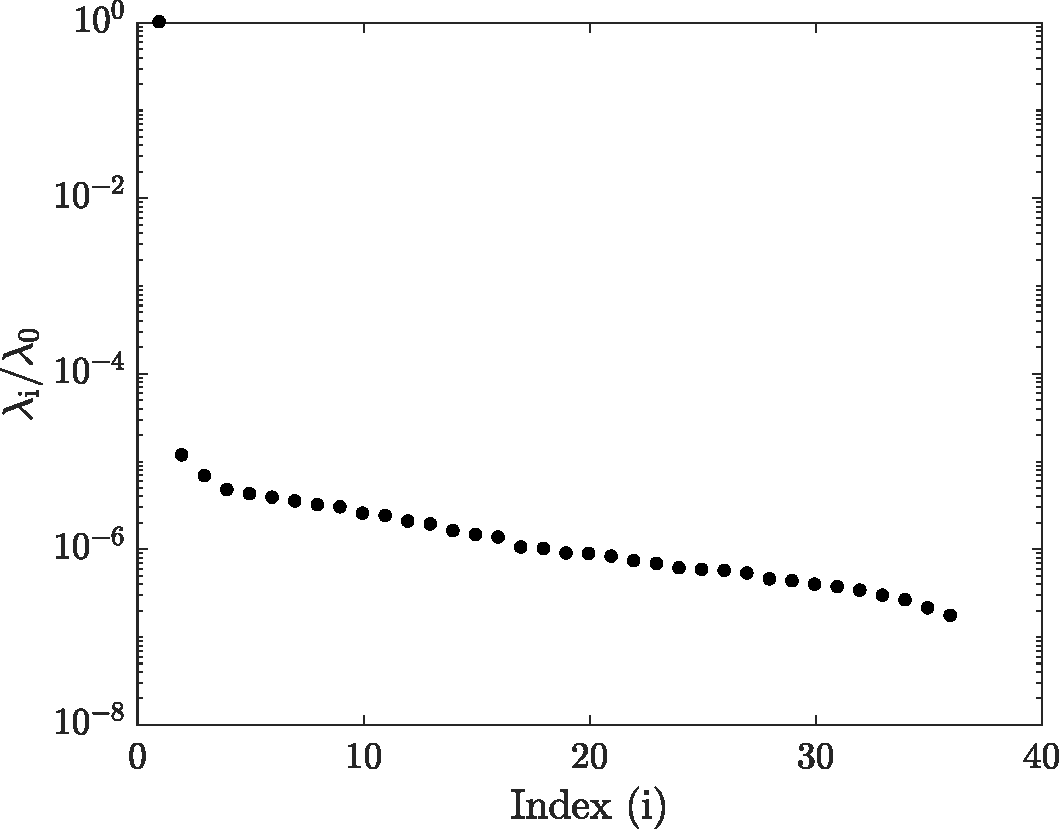
\includegraphics[width=0.4\textwidth]{./Figures/eig_plot_rev2}
  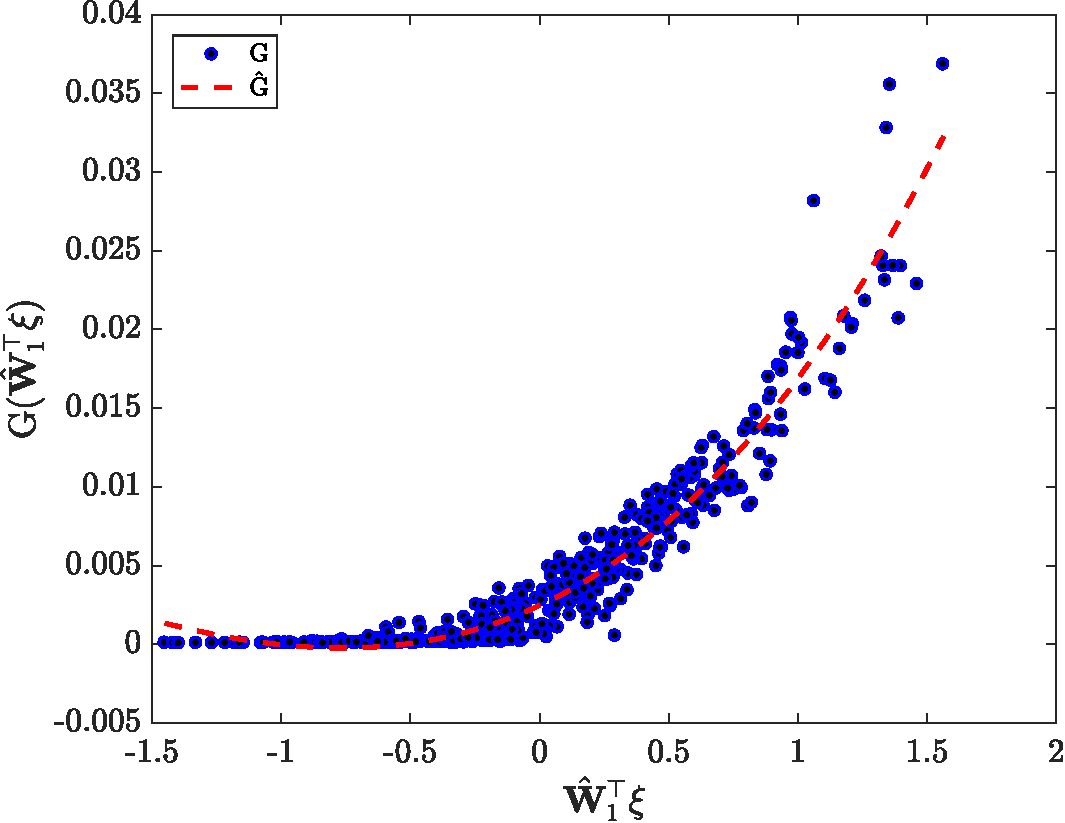
\includegraphics[width=0.4\textwidth]{./Figures/ssp_rev2}
\caption{Left: Eigenvalue spectrum of the matrix, $\hat{\bm{C}}$~(see~Eq.~8 in the paper). Right: Sufficient summary
plot~(SSP) in the active subspace. A polynomial fit (surrogate) is also shown.} 
\label{fig:as}
\end{center}
\end{figure}
%
The eigenvalue spectrum shows that $\frac{\lambda_1}{\lambda_2}\approx 10^{4}$ thereby indicating the presence of 
a 1-dimensional active subspace in this new regime as well. The SSP further confirms that the variability in ignition delay
is predominantly captured by a 1-dimensional active subspace. A polynomial fit of degree 3 is used as a surrogate for
estimating the global sensitivity measures of the individual rate-controlling parameters as well as the initial conditions:
$P_0$, $T_0$, and $\phi_0$. The sensitivity estimates based on activity scores are plotted in Figure~\ref{fig:as}.
 %
\begin{figure}[htbp]
 \begin{center}
  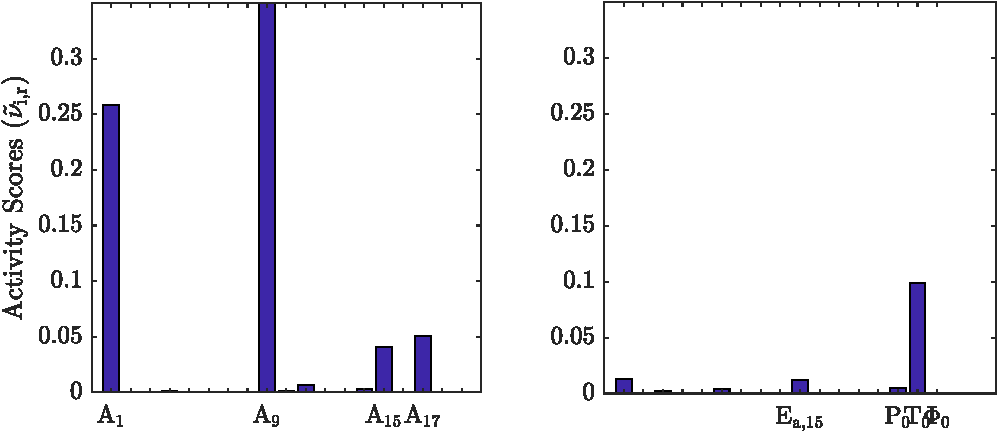
\includegraphics[width=0.85\textwidth]{./Figures/as_36D_rev2}
\caption{} 
\label{fig:as}
\end{center}
\end{figure}
%
It is observed that the ignition delay is mainly sensitive towards the rate parameters, $A_1$ and $A_9$. Sensitivity
towards $A_{15}$ and $A_{17}$ is also found to be significant. Among the initial conditions, $T_0$ is found to be
the most important. These findings for the newly considered regime are in fact consistent with the sensitivity results
obtained for the regime considered in the paper. Therefore, it is interesting to note that parametric sensitivities have
not changed much as a result of faster ignition due to increased initial pressure and temperature. 

Thus, the proposed methodology in the paper is successfully implemented in a regime of potential interest to
combustion scientists. It further highlights the robustness as well as the applicability of the framework to a wide
range of conditions for the kinetics application considered in this work. Moreover, the framework can be extended
to other systems
for the purpose of sensitivity analysis, uncertainty propagation, and parameter optimization. 

\end{enumerate}

\section*{Reviewer \#2}

\begin{enumerate}[wide, labelwidth=!, labelindent=0pt]
\item \referee{Fig 1: I don't think the why axis label is correct. There should be no 'log'. Same goes for the added blue text
on line 34 (page 12)}

The reviewer is correct in pointing out that there should be no $\log$ in the y axis label in
Figure~1 and the text in line 34 on Page~12.
The manuscript has been updated to reflect these corrections. 

\item \referee{page 7, line 55: typo 'Boltzmanm'}

The typo has been corrected in the revised manuscript. 

\item \referee{page 13, line 17: max is over j, it should be mentioned. Same comment for the beginning of Section 5.1, 
and for Figure 4.}

As suggested by the reviewer, the manuscript has been updated to indicate that the max is over `j' at the specified 
locations. 

\item \referee{page 13, line 19: no comma after 'both'}

This suggestion has been incorporated in the revised manuscript. 

\item \referee{page 13, line 23: typo 'as total of'$\rightarrow$'a total of'}

The typo has been rectified in the revised manuscript. 

\item \referee{Table 2: since mean and st.dev. are computed using 10$^4$ samples, I would only report two significant digits in 
the table, since sqrt(10$^4$)=10$^2$; the rest of the digits are within the noise estimate due to sampling. Of course this is only an 
estimate, but the authors could easily check by repeating the procedure with different valudation sets. As an alternative, to 
differentiate between the three cases, I'd recommend using a larger validation set, if possible.}

As suggested by the reviewer, Table~2 has been updated to report only up to two significant digits.

\item \referee{page 17 (and perhaps elsewhere): why is it called cross-validation and not just validation?}

The term ``cross-validation" has been used as opposed to ``validation" since an independent set of model evaluations
were used to assess the predictive accuracy of its surrogate. The term ``validation" is typically used in
situations where a model is tested for its predictability against experimental test data i.e. data not used for the purpose
of calibrating the model. 

\item \referee{Please improve the x-axis labels in Figure 7.}

Figure~7 has been updated to address the reviewer's concern. 

\end{enumerate}


%\bibliographystyle{elsarticle-num}
%\bibliography{REFER}
\end{document}
